% Shared style for all Git & GitHub lectures (same look as the N-body course)
\documentclass[11pt,a4paper]{article}
\usepackage[margin=2.3cm]{geometry}
\usepackage[T1]{fontenc}
\usepackage{lmodern}
\usepackage{upquote}   % straight quotes in monospaced text, so commands can be copied
\usepackage{microtype}
% keep '--' as two real hyphens in monospace text (commands like --version)
\DisableLigatures[-,<,>]{family=tt*}
\usepackage{booktabs,enumitem,graphicx,xcolor}
\usepackage{array}
\usepackage{needspace}
\usepackage{longtable}
\usepackage{float}
\usepackage{tikz}
\usetikzlibrary{arrows.meta,calc,positioning,decorations.pathreplacing,shapes.geometric,fit,backgrounds}
\usepackage[most]{tcolorbox}
\usepackage{listings}
\usepackage{fancyhdr}
\usepackage[colorlinks=true,linkcolor=blue!50!black,urlcolor=blue!50!black,citecolor=blue!50!black]{hyperref}

\setlength{\parindent}{0pt}
\setlength{\parskip}{0.6em}
\setlength{\abovecaptionskip}{4pt}
\usepackage[font=small,labelfont=bf]{caption}
\setlist{itemsep=0.2em,topsep=0.3em}

% ---------- colours ----------
\definecolor{cbg}{HTML}{F6F8FA}
\definecolor{ckw}{HTML}{0B5CAD}
\definecolor{ccm}{HTML}{6A737D}
\definecolor{cst}{HTML}{B5451B}
\definecolor{cpart}{HTML}{1F6FB2}
\definecolor{cheavy}{HTML}{C0392B}
\definecolor{cgreen}{HTML}{2E8B57}

% ---------- terminal listings ----------
% In a terminal session, lines starting with "$" are what YOU type.
% Everything else is what Git prints back.
\lstdefinestyle{term}{
  basicstyle=\ttfamily\small, backgroundcolor=\color{cbg},
  frame=single, rulecolor=\color{black!15}, showstringspaces=false,
  breaklines=true, columns=fullflexible, keepspaces=true,
  aboveskip=0.6em, belowskip=0.6em, xleftmargin=4pt, xrightmargin=4pt,
  literate={\$\ }{{\textcolor{cgreen}{\$\ }}}2,
  upquote=true
}
\lstset{style=term}
\newcommand{\code}[1]{\texttt{\small #1}}

% ---------- boxes ----------
\newtcolorbox{history}{colback=yellow!8,colframe=orange!60!black,
  title={History},fonttitle=\bfseries\small,left=4pt,right=4pt,top=2pt,bottom=2pt}
\newtcolorbox{quickfact}{colback=purple!4,colframe=purple!55!black,
  title={Quick fact},fonttitle=\bfseries\small,left=4pt,right=4pt,top=2pt,bottom=2pt}
\newtcolorbox{keyidea}{colback=blue!4,colframe=blue!50!black,
  title={Key idea},fonttitle=\bfseries\small,left=4pt,right=4pt,top=2pt,bottom=2pt}
\newtcolorbox{pitfall}{colback=red!4,colframe=red!55!black,
  title={Pitfall},fonttitle=\bfseries\small,left=4pt,right=4pt,top=2pt,bottom=2pt}
\newtcolorbox{tryit}{colback=teal!5,colframe=teal!55!black,
  title={Try it},fonttitle=\bfseries\small,left=4pt,right=4pt,top=2pt,bottom=2pt,breakable}
\newtcolorbox{homework}[1]{colback=green!4,colframe=green!40!black,
  title={Homework #1},fonttitle=\bfseries\small,left=4pt,right=4pt,top=2pt,bottom=2pt,
  breakable}
\newtcolorbox{goals}{colback=gray!6,colframe=gray!60!black,
  title={Learning goals},fonttitle=\bfseries\small,left=4pt,right=4pt,top=2pt,bottom=2pt}

% Solutions always start on a fresh page, behind a clear warning.
\newcommand{\solutionspage}{%
  \clearpage
  \begin{tcolorbox}[colback=red!6,colframe=red!60!black,halign=center]
    {\Large\bfseries Solutions}\\[0.3em]
    {\small Stop here if you have not tried the homework yet.\\
    Attempt every task first, run the checker, and only then read on.}
  \end{tcolorbox}
}

% ---------- Git diagram styles (TikZ) ----------
\tikzset{
  commit/.style={circle,draw=black!70,fill=blue!10,minimum size=7mm,inner sep=0pt,font=\scriptsize\ttfamily},
  newcommit/.style={commit,fill=orange!25,dashed},
  tag/.style={draw,rounded corners=2pt,font=\scriptsize\ttfamily,inner sep=2pt},
  branchtag/.style={tag,fill=green!15,draw=green!40!black},
  headtag/.style={tag,fill=yellow!30,draw=orange!70!black},
  remotetag/.style={tag,fill=purple!10,draw=purple!60!black},
  area/.style={draw,rounded corners,minimum height=11mm,minimum width=33mm,align=center,font=\small},
  cmdarrow/.style={->,thick,>=Stealth},
  link/.style={->,thick,>=Stealth,black!70},
}

% ---------- header ----------
\pagestyle{fancy}
\fancyhf{}
\renewcommand{\headrulewidth}{0.3pt}
\fancyfoot[C]{\thepage}
\newcommand{\lecturetitle}[3]{%
  \fancyhead[L]{\small\textit{Git \& GitHub from Zero}}
  \fancyhead[R]{\small Lecture #1}
  \begin{center}
    {\Large\bfseries Lecture #1}\\[0.4em]
    {\LARGE\bfseries #2}\\[0.4em]
    {\small #3}
  \end{center}
  \vspace{0.5em}
}

\tikzset{
  cbx/.style={draw,rounded corners,fill=blue!6,minimum width=1.9cm,minimum height=8mm,align=center,font=\scriptsize\ttfamily,inner sep=2pt},
  newc/.style={cbx,fill=green!15},
  oldc/.style={cbx,fill=black!8,draw=black!45,dashed,text=black!55}}
\begin{document}
\lecturetitle{8}{Rewriting History: Rebase and Cherry-Pick}{Replaying commits, tidying a branch, copying a single commit, and the one rule you must never break}

\begin{goals}
\begin{itemize}
  \item Explain what \code{git rebase} does, and how it differs from \code{git merge}.
  \item State the golden rule of rebasing and say why it exists.
  \item Clean up a messy branch with an interactive rebase (\code{fixup}, \code{reword}, \code{drop}).
  \item Push rewritten history safely with \code{--force-with-lease}.
  \item Copy a single commit to another branch with \code{git cherry-pick}.
  \item Resolve a conflict in the middle of a rebase.
\end{itemize}
\end{goals}

\section{Why rewrite history?}

Real work is messy. You commit ``wip'' at five o'clock, ``fix typo'' ten minutes later, and ``oops'' after that. Before others read your branch you would like a clean story: one commit per idea, sensible messages, and a history that ends on top of the latest \code{main} instead of forking off an old one.

Git lets you \emph{rewrite} history for that purpose. In Lecture 3 you already did a tiny version (\code{git commit --amend}). This lecture adds the big tools. They are powerful and, used wrongly, they cause exactly the confusion that Lecture 6 warned about, so we learn the safety rule together with the tools.

We use a practice repository again, with a ``server'' folder that plays the role of GitHub. From the course folder:

\begin{lstlisting}
$ bash codeHints/L08/setup_demo8.sh
$ cd practice/demo8
$ git log --oneline --graph --all --decorate
* e04fe10 (HEAD -> main, origin/main, origin/HEAD) Add muffin recipe
| * 1f323f7 (origin/syrup) Pancakes with syrup
|/
| * 889b766 (origin/sale) Add sale banner
|/
| * 336710f (origin/cookies) fix typo in cookies
| * a7dfee0 wip
| * 45b2a27 Add cookie recipe
|/
* 699939b Add recipes
* 89ee60b Add README
\end{lstlisting}

The branch \code{cookies} has three messy commits and forked from \code{Add recipes}; meanwhile \code{main} moved on by one commit. The branches \code{sale} and \code{syrup} are for later. (The IDs of the starting commits match yours; the IDs of commits that \emph{you} create below will differ, as always.) Set your identity once in this clone if you have not set it globally: \code{git config user.name} and \code{git config user.email}.

\section{Rebase: replaying commits on a new base}

You know one way to bring \code{cookies} up to date with \code{main}: merge \code{main} into it (Lecture 5). (\code{cookies} is a branch that only \emph{you} work on, which is what makes the rewriting below allowed; Section~\ref{sec:golden} explains why that matters.) \textbf{Rebase} does it differently. It takes your commits, one at a time, and \emph{replays} them on top of the new tip of \code{main}, as if you had started your work from there.

\begin{lstlisting}
$ git switch cookies
branch 'cookies' set up to track 'origin/cookies'.
$ git rebase main
Successfully rebased and updated refs/heads/cookies.
$ git log --oneline --graph --decorate -5
* 5bfcea2 (HEAD -> cookies) fix typo in cookies
* dd806cd wip
* 539c33d Add cookie recipe
* e04fe10 (origin/main, origin/HEAD, main) Add muffin recipe
* 699939b Add recipes
\end{lstlisting}

(Git also prints progress lines such as \code{Rebasing (2/3)}, left out here.) The history is now one straight line: no fork, no merge commit. But the \emph{old} commits are not gone; the server's \code{origin/cookies} still points at them:

\begin{lstlisting}
$ git log --oneline --graph --all --decorate
* 5bfcea2 (HEAD -> cookies) fix typo in cookies
* dd806cd wip
* 539c33d Add cookie recipe
* e04fe10 (origin/main, origin/HEAD, main) Add muffin recipe
| * 336710f (origin/cookies) fix typo in cookies
| * a7dfee0 wip
| * 45b2a27 Add cookie recipe
|/
* 699939b Add recipes
\end{lstlisting}

Two versions of the same work now exist: your new copies, and the originals that the server still holds. Remember this picture; it explains why the push later is refused.

\begin{figure}[H]
\centering
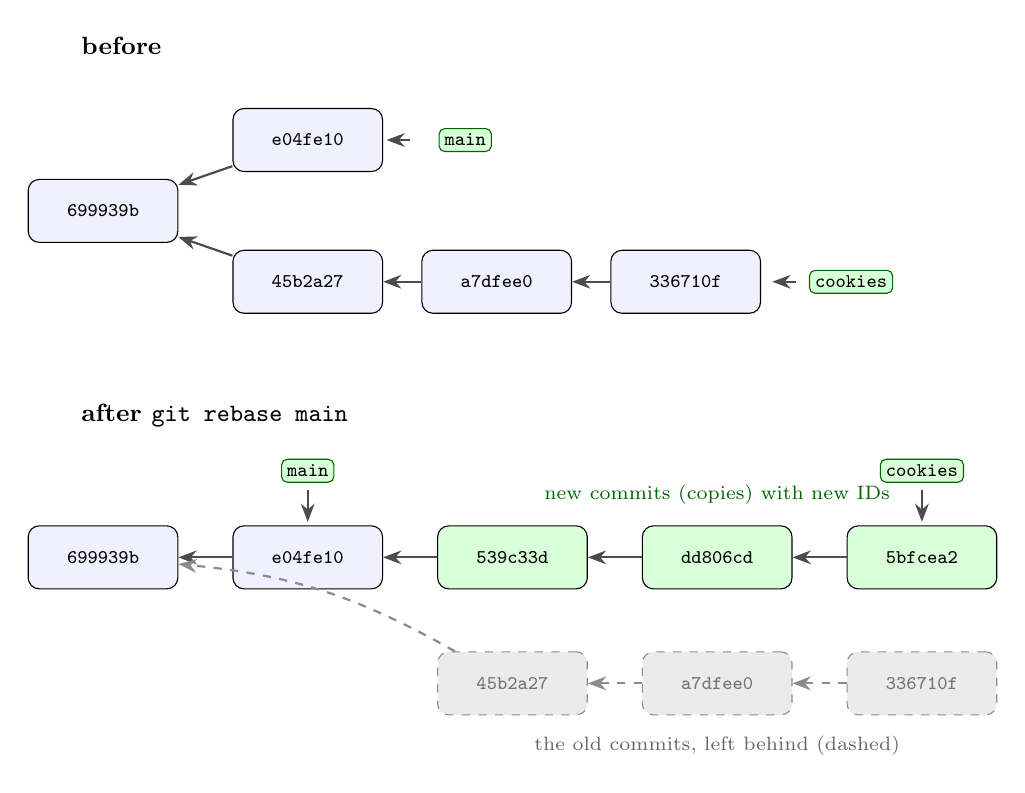
\begin{tikzpicture}
  \node[font=\small\bfseries,anchor=west] at (-0.4,2.1) {before};
  \node[cbx] (r2) at (0,0) {699939b};
  \node[cbx] (r3) at (2.6,0.9) {e04fe10};
  \node[cbx] (c1) at (2.6,-0.9) {45b2a27}; \node[cbx] (c2) at (5.0,-0.9) {a7dfee0}; \node[cbx] (c3) at (7.4,-0.9) {336710f};
  \draw[link] (r3)--(r2); \draw[link] (c1)--(r2); \draw[link] (c2)--(c1); \draw[link] (c3)--(c2);
  \node[branchtag] at (4.6,0.9) {main}; \draw[link] (3.9,0.9)--(3.6,0.9);
  \node[branchtag] at (9.5,-0.9) {cookies}; \draw[link] (8.8,-0.9)--(8.5,-0.9);
  \node[font=\small\bfseries,anchor=west] at (-0.4,-2.6) {after \code{git rebase main}};
  \node[cbx] (q2) at (0,-4.4) {699939b};
  \node[cbx] (q3) at (2.6,-4.4) {e04fe10};
  \node[newc] (n1) at (5.2,-4.4) {539c33d}; \node[newc] (n2) at (7.8,-4.4) {dd806cd}; \node[newc] (n3) at (10.4,-4.4) {5bfcea2};
  \draw[link] (q3)--(q2); \draw[link] (n1)--(q3); \draw[link] (n2)--(n1); \draw[link] (n3)--(n2);
  \node[branchtag] at (2.6,-3.3) {main}; \draw[link] (2.6,-3.55)--(2.6,-3.95);
  \node[branchtag] at (10.4,-3.3) {cookies}; \draw[link] (10.4,-3.55)--(10.4,-3.95);
  \node[oldc] (p1) at (5.2,-6.0) {45b2a27}; \node[oldc] (p2) at (7.8,-6.0) {a7dfee0}; \node[oldc] (p3) at (10.4,-6.0) {336710f};
  \draw[link,black!45,dashed] (p1) to[bend right=12] (q2); \draw[link,black!45,dashed] (p2)--(p1); \draw[link,black!45,dashed] (p3)--(p2);
  \node[font=\scriptsize,text=green!40!black,anchor=south] at (7.8,-3.85) {new commits (copies) with new IDs};
  \node[font=\scriptsize,text=black!60,anchor=north] at (7.8,-6.55) {the old commits, left behind (dashed)};
\end{tikzpicture}
\caption{Rebase replays the three commits on top of \code{main}. The copies have the same changes and messages but \emph{new IDs}, because their parent is different. The old commits (dashed, \code{45b2a27} and so on) are left behind.}
\label{fig:rebase}
\end{figure}

\begin{keyidea}
A commit's ID depends on its parent. If you move a commit onto a different parent, you get a \emph{different commit}: same change, same message, new ID. Rebase therefore does not move commits; it \textbf{creates copies} and abandons the old ones. That is what ``rewriting history'' means. (You have seen it before: \code{git commit --amend} in Lecture 3 also gave you a new ID.)
\end{keyidea}

\subsection{Merge or rebase?}

\begin{center}
\small
\begin{tabular}{@{}l >{\raggedright\arraybackslash}p{4.6cm} >{\raggedright\arraybackslash}p{4.6cm}@{}}
\toprule
 & \code{git merge main} & \code{git rebase main} \\
\midrule
History shape & keeps the fork, adds a merge commit & one straight line \\
Existing commits & untouched & copied, with new IDs \\
Conflicts & resolved once, in the merge & possibly once per replayed commit \\
Safe on shared branches & yes & \textbf{no} (see the golden rule) \\
\bottomrule
\end{tabular}
\end{center}

Neither is ``right''. Merge records exactly what happened. Rebase gives a tidier story. Many teams use rebase for their \emph{own} work in progress and merge for the finished result.

\section{Conflicts during a rebase}\label{sec:conflicts}

Because rebase replays commits one by one, a conflict can appear in the middle. Rebase the branch \code{syrup}: it edits the same line that \code{main}'s newest commit sits right next to.

\Needspace{20\baselineskip}
\begin{lstlisting}
$ git switch syrup
branch 'syrup' set up to track 'origin/syrup'.
$ git rebase main
Auto-merging recipes.txt
CONFLICT (content): Merge conflict in recipes.txt
error: could not apply 1f323f7... Pancakes with syrup
hint: Resolve all conflicts manually, mark them as resolved with
hint: "git add/rm <conflicted_files>", then run "git rebase --continue".
hint: You can instead skip this commit: run "git rebase --skip".
hint: To abort and get back to the state before "git rebase", run "git rebase --abort".
$ cat recipes.txt
<<<<<<< HEAD
Pancakes: flour, milk, eggs
Muffins: flour, milk
=======
Pancakes: flour, milk, eggs, syrup
>>>>>>> 1f323f7 (Pancakes with syrup)
\end{lstlisting}

The rebase is paused, halfway, exactly like a conflicted merge. \code{git status} confirms it, and you will see that you are temporarily ``on no branch'':

\begin{lstlisting}
$ git status
interactive rebase in progress; onto e04fe10
Last command done (1 command done):
   pick 1f323f7 Pancakes with syrup
...
$ git status -sb
## HEAD (no branch)
UU recipes.txt
\end{lstlisting}

That is normal during a rebase. The procedure is the one from Lecture 5, with a different last step:

\begin{enumerate}
  \item Edit the file: choose or combine, remove the three marker lines.
  \item \code{git add recipes.txt} (``resolved'').
  \item \code{git rebase --continue} (not \code{git commit}). Git then replays the next commit, if any. \emph{An editor may open} showing the commit's original message: just save and close it (see the box on editors below).
\end{enumerate}

\begin{lstlisting}
$ printf 'Pancakes: flour, milk, eggs, syrup\nMuffins: flour, milk\n' > recipes.txt
$ git add recipes.txt
$ git rebase --continue
Successfully rebased and updated refs/heads/syrup.
\end{lstlisting}

\begin{pitfall}
\textbf{The editor.} Git sometimes opens a text editor, often \code{vim}, which does not accept normal typing. Survival recipe: press \code{i} to start typing; move with the arrow keys; delete with Backspace or Delete; press \code{Esc}; type \code{:wq} and press Enter to save and quit. (If \code{:wq} just shows up as text, you were still in insert mode: press \code{Esc} first.) If the editor shows a message you only need to accept, do just \code{Esc}, \code{:wq}, Enter. In \code{nano}, save with Ctrl+O then Enter and quit with Ctrl+X. You can choose another editor once and for all, for example \code{git config --global core.editor "nano"} or, for VS Code, \code{git config --global core.editor "code --wait"}.
\end{pitfall}

\begin{pitfall}
\textbf{The two sides are swapped compared with a merge.} During a rebase, the part above \code{=======} (labelled \code{HEAD}) is the branch you are rebasing \emph{onto}, here \code{main}. The part below is \emph{your own commit} being replayed. Read the labels, not the order, and keep what you want.
\end{pitfall}

\Needspace{9\baselineskip}
Your three escape hatches while a rebase is paused:

\begin{center}
\small
\begin{tabular}{@{}l >{\raggedright\arraybackslash}p{9.4cm}@{}}
\toprule
Command & Effect \\
\midrule
\code{git rebase --continue} & After resolving: go on with the next commit. \\
\code{git rebase --abort} & Cancel everything. The branch is exactly as before you started. Always safe. \\
\code{git rebase --skip} & Drop the commit that conflicts and go on (its change is lost). \\
\bottomrule
\end{tabular}
\end{center}

\section{Interactive rebase: tidying your commits}

The most useful form of rebase lets you \emph{edit the list of commits}. Our \code{cookies} branch has the story ``Add cookie recipe, wip, fix typo''. We want a single commit. Start an interactive rebase onto \code{main}:

\begin{lstlisting}
$ git switch cookies
$ git rebase -i main
\end{lstlisting}

(You may also say \code{git rebase -i HEAD\textasciitilde{}3}: ``the last three commits''.) Git opens your editor with a \textbf{todo list}, one command per line, \emph{oldest commit first} (the opposite of \code{git log}, which shows the newest first). In short: \code{fixup} means ``squash this commit into the one above and throw away its message''; the table below lists all commands.

\begin{lstlisting}
pick 539c33d Add cookie recipe
pick dd806cd wip
pick 5bfcea2 fix typo in cookies

# Rebase e04fe10..5bfcea2 onto e04fe10 (3 commands)
#
# Commands:
# p, pick <commit> = use commit
# r, reword <commit> = use commit, but edit the commit message
# e, edit <commit> = use commit, but stop for amending
# s, squash <commit> = use commit, but meld into previous commit
# f, fixup <commit> = like "squash" but keep only the previous commit's message
# d, drop <commit> = remove commit
# (...more commands and a warning about deleted lines...)
\end{lstlisting}

(Your Git may word these comment lines slightly differently.)

Change the word at the start of a line to tell Git what to do with that commit: in the editor, delete \code{pick} and type the new word (\code{fixup}, or just its letter \code{f}; \code{r} for \code{reword}, \code{s}, \code{d}). To fold the second and third commit into the first, replace \code{pick} by \code{fixup} on those lines, then save and close the editor (\code{Esc}, \code{:wq}, Enter; see the box on editors in Section~\ref{sec:conflicts}):

\begin{lstlisting}
pick 539c33d Add cookie recipe
fixup dd806cd wip
fixup 5bfcea2 fix typo in cookies
\end{lstlisting}

\begin{lstlisting}
$ git log --oneline --decorate -4
8d96fcc (HEAD -> cookies) Add cookie recipe
e04fe10 (origin/main, origin/HEAD, main) Add muffin recipe
699939b Add recipes
89ee60b Add README
\end{lstlisting}

Three commits became one, with the combined changes and the first message.

\begin{center}
\small
\begin{tabular}{@{}l >{\raggedright\arraybackslash}p{10.2cm}@{}}
\toprule
Command & What it does \\
\midrule
\code{pick} & Keep the commit as it is. \\
\code{reword} & Keep the changes, but let me edit the message (the editor opens again). \\
\code{squash} & Merge into the previous commit and let me combine both messages. \\
\code{fixup} & Merge into the previous commit and discard this message. \\
\code{drop} & Delete the commit (or delete the line). Its changes are gone. \\
\code{edit} & Stop after this commit so I can change it (then \code{git rebase --continue}). \\
\bottomrule
\end{tabular}
\end{center}

You can also \emph{reorder} commits by moving lines. The commits are replayed from top to bottom. Things that go wrong: a \code{fixup} on the \emph{first} line fails (``cannot fixup without a previous commit''); a misspelt command word stops the rebase (fix the list with \code{git rebase --edit-todo}); and if you quit the editor without changing anything, Git simply replays every commit as \code{pick}. To cancel before you finish: delete every line of the list and save, or run \code{git rebase --abort} later.

\begin{quickfact}
Shortcut for the future: \code{git commit --fixup <id>} makes a commit that is marked as a fix for an earlier commit, and \code{git rebase -i --autosquash main} then arranges and folds it automatically. You do not need it now.
\end{quickfact}

\section{The golden rule}\label{sec:golden}

\begin{keyidea}
\textbf{Never rebase commits that other people already have.} Rebase only commits that exist solely on your computer, or on a branch that only you use.
\end{keyidea}

Why? Rebasing replaces commits with copies. If a teammate has the \emph{old} commits and you publish the \emph{copies}, the two of you now disagree about what the history is:

\begin{figure}[H]
\centering
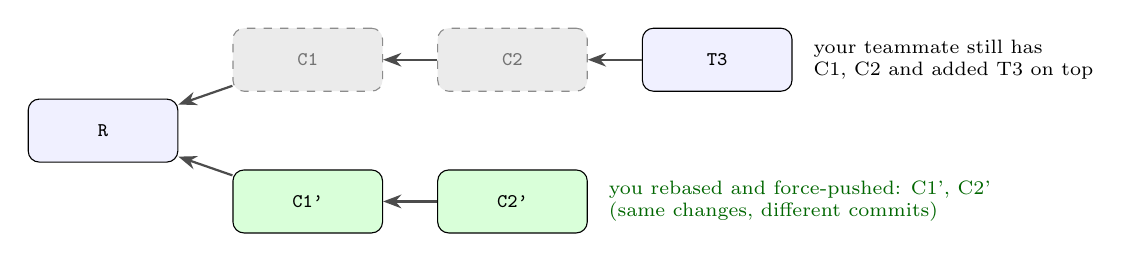
\begin{tikzpicture}
  \node[cbx] (a) at (0,0) {R};
  \node[oldc] (o1) at (2.6,0.9) {C1}; \node[oldc] (o2) at (5.2,0.9) {C2}; \node[cbx] (t3) at (7.8,0.9) {T3};
  \node[newc] (n1) at (2.6,-0.9) {C1'}; \node[newc] (n2) at (5.2,-0.9) {C2'};
  \draw[link] (o1)--(a); \draw[link] (o2)--(o1); \draw[link] (t3)--(o2);
  \draw[link] (n1)--(a); \draw[link] (n2)--(n1);
  \node[font=\scriptsize,anchor=west,align=left] at (8.9,0.9) {your teammate still has\\C1, C2 and added T3 on top};
  \node[font=\scriptsize,anchor=west,align=left,text=green!40!black] at (6.3,-0.9) {you rebased and force-pushed: C1', C2'\\(same changes, different commits)};
\end{tikzpicture}
\caption{The teammate's \code{T3} sits on the old \code{C2}, which no longer exists on the server. Combining the two histories duplicates \code{C1} and \code{C2} and invites conflicts that nobody caused.}
\label{fig:golden}
\end{figure}

What your teammate sees: after they \code{git pull}, Git finds your new \code{C1'} and \code{C2'} on the server and their own \code{C1} and \code{C2} locally, which look like \emph{different} commits. They get a merge full of duplicated changes or conflicts that nobody caused, and your rewritten history spreads confusion across the team.

Commits you have only locally are safe to rewrite, and so is a branch that you alone work on, even if you pushed it, \emph{as long as you are sure no one else has fetched it}. Never rewrite \code{main} or a branch your team shares.

\subsection{Pushing rewritten history}

After the rebase and the tidy-up of \code{cookies}, your local branch has copies and the server still has the originals (the picture after the first rebase). A normal push is refused, because it would not just add commits, it would replace them:

\begin{lstlisting}
$ git push
To github.com:you/recipes.git
 ! [rejected]        cookies -> cookies (non-fast-forward)
error: failed to push some refs to 'github.com:you/recipes.git'
hint: Updates were rejected because the tip of your current branch is behind
\end{lstlisting}

This is the situation for which beginners reach for \code{git push --force}, which overwrites the remote branch \emph{unconditionally}. Use the safer cousin instead:

\begin{lstlisting}
$ git push --force-with-lease
To github.com:you/recipes.git
 + 336710f...8d96fcc cookies -> cookies (forced update)
\end{lstlisting}

\textbf{\code{--force-with-lease}} means ``replace the remote branch, but \emph{only if it is still where my last \code{git fetch} saw it}'' (your \code{origin/cookies}). If someone pushed in the meantime, it refuses, and you find out before you destroy their work. To try it yourself on the branch \code{sale}: rewrite its commit, let a friend push to it, then push:

\Needspace{9\baselineskip}
\begin{lstlisting}
$ git switch sale
$ git commit --amend -m "Add sale banner (reworded)"   # fine here: a practice branch
$ bash codeHints/L08/friend8.sh sale          # a friend pushes (course folder)
$ git push --force-with-lease
To github.com:you/recipes.git
 ! [rejected]        sale -> sale (stale info)
error: failed to push some refs to 'github.com:you/recipes.git'
\end{lstlisting}

``Stale info'' means: the remote branch has moved since you last looked. Do \emph{not} escalate to \code{--force}, which would erase your friend's commit. Instead fetch, read what arrived (\code{git log origin/sale}), and talk to your friend. Note the limit of the lease: after a \code{git fetch} (also an automatic one by your editor), Git has seen the friend's commit, and a later \code{--force-with-lease} would overwrite it. The lease is a seat belt, \emph{not} permission to rebase a shared branch.

\begin{pitfall}
Even \code{--force-with-lease} must not be used on \code{main} or any shared branch. Hosting sites can forbid it with \emph{branch protection}; Lecture 9 shows how.
\end{pitfall}

\section{Cherry-pick: copying one commit}

Sometimes you want \emph{one} commit from another branch, not the whole branch. The server's branch \code{sale} has a commit \code{Add sale banner}, and \code{main} should get it now. (If you tried the amend demo above, your local \code{sale} holds a \emph{reworded copy}; the original commit \code{889b766} is still on \code{origin/sale}, so use that ID exactly as shown.)

\Needspace{11\baselineskip}
\begin{lstlisting}
$ git switch main
$ git cherry-pick 889b766
[main 26e9c4f] Add sale banner
 Author: Practice User <practice@example.com>
 Date: Wed Nov 6 09:00:00 2024 +0000
 1 file changed, 1 insertion(+)
 create mode 100644 banner.txt
\end{lstlisting}

\begin{figure}[H]
\centering
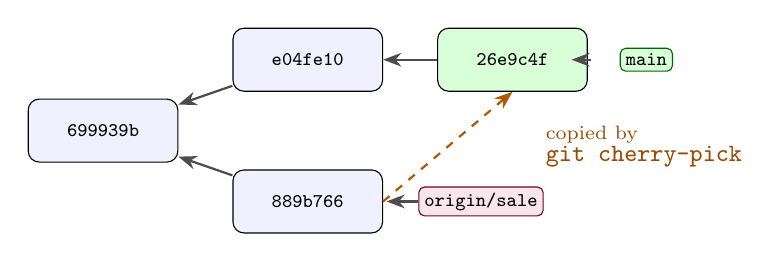
\begin{tikzpicture}
  \node[cbx] (r) at (0,0) {699939b};
  \node[cbx] (m) at (2.6,0.9) {e04fe10}; \node[cbx] (s) at (2.6,-0.9) {889b766};
  \node[newc] (c) at (5.2,0.9) {26e9c4f};
  \draw[link] (m)--(r); \draw[link] (s)--(r); \draw[link] (c)--(m);
  \draw[->,thick,>=Stealth,dashed,orange!70!black] (s.east) -- (c.south);
  \node[font=\scriptsize,align=left,orange!60!black,anchor=west] at (5.5,-0.2) {copied by\\\code{git cherry-pick}};
  \node[branchtag] at (6.9,0.9) {main}; \draw[link] (6.2,0.9)--(5.95,0.9);
  \node[remotetag] at (4.8,-0.9) {origin/sale}; \draw[link] (4.0,-0.9)--(3.6,-0.9);
\end{tikzpicture}
\caption{Cherry-pick creates a \emph{copy} of \code{889b766} on top of \code{main}. The original stays on \code{sale}.}
\label{fig:cherry}
\end{figure}

The copy has a new ID and parent, but the same change, message, author and original date. If the change does not apply cleanly you get a conflict, which you resolve as before, then finish with \code{git cherry-pick --continue} (or cancel with \code{git cherry-pick --abort}). Adding \code{-x} appends ``(cherry picked from commit \dots)'' to the message, which helps later.

Typical uses:
\begin{itemize}
  \item \textbf{A hotfix} made on one branch that must also go to \code{main}.
  \item \textbf{A commit made on the wrong branch} (the mistake warned about in Lecture 4). Illustration only (do not type this now): you committed ``snickerdoodle'' on \code{main} but it belongs on \code{cookies}.
\end{itemize}

\begin{lstlisting}
$ git switch main
$ git log --oneline -1
9f74ed1 Add snickerdoodle (wrong branch)
$ git switch cookies
$ git cherry-pick 9f74ed1
[cookies 4be0c21] Add snickerdoodle (wrong branch)
\end{lstlisting}

The commit is now on the right branch. Its copy on the wrong branch must still be removed; that needs \code{git reset}, introduced in Lecture 10. (The ID of your copy will differ.)

\begin{pitfall}
Cherry-pick \emph{duplicates} a change. If you later merge the whole branch as well, Git usually recognises the same change and copes, but long-lived copies cause confusing conflicts. Use it for single, deliberate commits, not as a way to move branches around.
\end{pitfall}

\section{Pulling with rebase}

In Lecture 6 a push was rejected because the server had a commit you lacked, and \code{git pull} asked you how to reconcile. Merge was one answer. \textbf{Rebase} is the other: put your unpushed commits \emph{on top of} what the server has.

In the demo, your cherry-picked \code{Add sale banner} is a local commit on \code{main} that you have not pushed. Let a friend push to \code{main} (from the course folder: \code{bash codeHints/L08/friend8.sh main}), then:

\Needspace{14\baselineskip}
\begin{lstlisting}
$ git push
 ! [rejected]        main -> main (fetch first)
$ git pull --rebase
Successfully rebased and updated refs/heads/main.
$ git log --oneline --graph --decorate -4
* 57a80aa (HEAD -> main) Add sale banner
* 2e17653 (origin/main, origin/HEAD) Add friend news
* e04fe10 Add muffin recipe
* 699939b Add recipes
$ git push
   2e17653..57a80aa  main -> main
\end{lstlisting}

The result is a straight line with no merge commit. This is safe, because your local commit had not been shared yet, so replacing it by a copy hurts nobody. You can make it the default with \code{git config --global pull.rebase true}; the choice you made in Lecture 6 (\code{false}, merge) was equally valid.

\section{Rebase and GitHub}

Lecture 7 offered three merge buttons. You can now read two of them: \textbf{Squash and merge} is like the \code{squash}/\code{fixup} of this lecture done by GitHub (many commits become one), and \textbf{Rebase and merge} is a rebase done by GitHub (new commits again, hence the \code{-d} surprise).

A pull request that has fallen behind \code{main} can be brought up to date by merging \code{main} into it (always safe) or by rebasing it and pushing with \code{--force-with-lease}. Choose the rebase \emph{only} when you are the sole author of the branch.

\begin{quickfact}
Rebased commits are not destroyed at once. Git remembers where your branch was before, so even a disastrous rebase can usually be undone. Lecture 10 shows how with the \emph{reflog}. Until then, \code{git rebase --abort} is your friend during a rebase.
\end{quickfact}

\Needspace{12\baselineskip}
\section{Homework 8}

\begin{homework}{8: Clean up and ship}
The setup script creates \code{practice/hw8\_server.git}, a shared ``server'' repository with three branches: \code{main}, \code{feature} (five messy commits, already pushed) and \code{hotfix} (one commit). From the course folder:
\begin{lstlisting}
$ bash codeHints/L08/setup_hw8.sh
$ cd practice
\end{lstlisting}
You are the only person working on \code{feature}, so rewriting it is allowed. Rebase and cherry-pick need your Git identity: run \code{git config user.name} and \code{git config user.email} in the clone if you have not set them globally. Do the tasks in order. To start over: \code{setup\_hw8.sh --reset} from the course folder.

\begin{description}[leftmargin=1.2em,style=nextline]
\item[8.1 Look] Clone the server into \code{hw8}, go in, and run \code{git log --oneline --graph --all --decorate}.
\item[8.2 Tidy and rebase] On \code{feature} run \code{git rebase -i main}. Turn the five commits into \emph{two}: fold the \code{wip} and \code{fix typo} commits into \code{Add greeting}, fold \code{oops} into \code{add farewell}, and \emph{reword} \code{add farewell} to \code{Add farewell}. The first commit conflicts in \code{README.md}: keep \emph{both} added lines (\code{Maintained by the team.} and \code{Usage: run the greeter.}), remove the markers, \code{git add README.md}, and \code{git rebase --continue}. An editor opens \emph{twice} during this task (first for the conflicted commit's message, later for the reword): in both, save and close, and change the text only for the reword.
\item[8.3 Check] \code{git log --oneline --reverse main..feature} (\code{--reverse}: oldest first; \code{main..feature}: the commits on \code{feature} that \code{main} lacks) must show exactly two commits, \code{Add greeting} and then \code{Add farewell}, on top of \code{main}'s newest commit.
\item[8.4 Publish] Try a plain \code{git push} and read the rejection. Then push with \code{git push --force-with-lease}.
\item[8.5 Cherry-pick] Switch to \code{main}. Find the commit on \code{origin/hotfix} (\code{git log origin/hotfix}) and copy it onto \code{main} with \code{git cherry-pick}. Push \code{main}. (\code{main} must stay a straight line: no merge.)
\item[8.6 Questions] In \code{practice/hw8\_answers.txt} (next to \code{hw8}, created with \code{printf} or \code{echo}) write three lines: \code{shared-rebase=<yes or no>} (is it fine to rebase commits your teammates have already pulled?), \code{safer-force=<option>} (the safer alternative to \code{--force}), and \code{new-ids=<merge or rebase>} (which of the two creates copies of your commits with new IDs?).
\end{description}

\textbf{Check yourself:} from the course folder run \code{bash codeHints/L08/check\_hw8.sh}. All \code{PASS}, then compare with the solutions at the end of this lecture (or in \code{solutions/L08/}).
\end{homework}

\section{Summary}

\begin{itemize}
  \item Rebase replays your commits on a new base, creating copies with new IDs: a straight history instead of a fork. A rebase conflict is resolved with \code{add} and \code{git rebase --continue}; \code{--abort} undoes it all.
  \item Golden rule: never rebase commits others already have. After rebasing your own pushed branch, use \code{--force-with-lease}, never plain \code{--force}.
  \item \code{git rebase -i}: \code{pick}, \code{reword}, \code{squash}, \code{fixup}, \code{drop}, reorder.
  \item \code{git cherry-pick} copies one commit onto the current branch. \code{git pull --rebase} avoids a merge commit when you only have local commits. (\emph{Pro Git}, Chapters 3.6, 7.6.)
\end{itemize}


\solutionspage

\section*{Solutions to Homework 8}

\begin{lstlisting}
$ bash codeHints/L08/setup_hw8.sh
$ cd practice
$ git clone hw8_server.git hw8
$ cd hw8
$ git log --oneline --graph --all --decorate
$ git switch feature
$ git rebase -i main
\end{lstlisting}

The editor opens with the five commits, oldest first (your IDs differ from here on):

\begin{lstlisting}
pick 74e9302 Add greeting
pick b8385c7 wip
pick c59f243 fix typo
pick 3b4d390 add farewell
pick 83ae7a6 oops
\end{lstlisting}

Change the first word of lines 2 to 5, save and close:

\begin{lstlisting}
pick 74e9302 Add greeting
fixup b8385c7 wip
fixup c59f243 fix typo
reword 3b4d390 add farewell
fixup 83ae7a6 oops
\end{lstlisting}

Git replays \code{Add greeting} first and stops with a conflict in \code{README.md} (you also see \code{HEAD (no branch)} in \code{git status}: normal during a rebase), because \code{main}'s newest commit also added a line there. In the file, the part above \code{=======} is \code{main}'s line and the part below is yours; keep both:

\begin{lstlisting}
# Greeter
Maintained by the team.
Usage: run the greeter.
\end{lstlisting}

\begin{lstlisting}
$ git add README.md
$ git rebase --continue
        # editor 1: message of "Add greeting": save and close
        # editor 2 (reword): change "add farewell" to "Add farewell"
$ git log --oneline --reverse main..feature
$ git push                       # rejected (non-fast-forward): expected
$ git push --force-with-lease
$ git log --oneline origin/hotfix -1
$ git switch main
$ git cherry-pick <that-id>
$ git push
$ printf 'shared-rebase=no\nsafer-force=force-with-lease\nnew-ids=rebase\n' \
    > ../hw8_answers.txt
\end{lstlisting}

\textbf{8.2.} \code{fixup} merges a commit into the one above and keeps the \emph{upper} message, so \code{wip} and \code{fix typo} disappear into \code{Add greeting}, and \code{oops} into \code{Add farewell}. \code{reword} stops once more so that you can fix the capital letter. If you used \code{squash} instead of \code{fixup}, Git opens an editor with combined messages, and you must delete the extra ones, otherwise the checker finds the wrong messages.

\textbf{8.3.} Two commits, \code{Add greeting} and \code{Add farewell}, on top of \code{Update README}. If \code{git log --oneline main..feature} shows five commits, you ran a plain rebase without \code{-i} or forgot to edit the list.

\textbf{8.4.} The rebase created copies of the commits, so the server's \code{feature} (with the old five) is no longer an ancestor of yours, and a normal push is rejected. \code{--force-with-lease} is allowed to replace it because the server's branch is exactly where you last saw it.

\textbf{8.5.} \code{git cherry-pick} copies the hotfix commit onto \code{main}: a \emph{new} commit with the same change and message. The original stays on \code{hotfix}. \code{main} remains a straight line of four commits. (Merging \code{hotfix} would add the original commit and a merge commit, which the checker rejects.)

\textbf{8.6.} \code{shared-rebase=no} (golden rule), \code{safer-force=force-with-lease}, \code{new-ids=rebase} (merge keeps all existing commits and only adds one).

\Needspace{8\baselineskip}
\textbf{Common mistakes.}
\begin{itemize}
  \item Merging \code{main} into \code{feature} instead of rebasing: the history keeps five messy commits plus a merge commit.
  \item Leaving the rebase unfinished (after a conflict you must \code{git add} and \code{git rebase --continue}). \code{git status} says \code{rebase in progress}; the checker's last check fails until you finish or \code{git rebase --abort}.
  \item Using plain \code{git push --force}. It works here, but it is exactly the habit the lecture warns against; use \code{--force-with-lease}.
  \item Stuck in the vim editor: press \code{Esc}, type \code{:wq}, press Enter. (\code{:q!} quits \emph{without saving}, which does not cancel a rebase: with an unchanged todo list every commit is simply replayed.) To cancel a rebase, run \code{git rebase --abort}, or delete all lines of the todo list and save.
\end{itemize}


\end{document}
